\clearpage
\makeatletter
\efloat@restorefloats
\makeatother


\begin{appendix}
\section{}
\hypertarget{supplimentary-analysis}{%
\subsection{Supplimentary Analysis}\label{supplimentary-analysis}}

\begin{table}[h]

\begin{center}
\begin{threeparttable}

\caption{\label{tab:tabDesAppB}Descriptive Statistics for Unmerged response options}

\begin{tabular}{ccccccc}
\toprule
 & \multicolumn{1}{c}{Mean} & \multicolumn{1}{c}{SD} & \multicolumn{1}{c}{Skew} & \multicolumn{1}{c}{Kurtosis} & \multicolumn{1}{c}{Shapiro-Wilk Statistics} & \multicolumn{1}{c}{Item-Total Correlation}\\
\midrule
Item1 & 2.16 & 1.51 & 0.49 & -0.86 & 0.90* & .21\\
Item2 & 2.76 & 1.75 & -0.10 & -1.42 & 0.88* & .20\\
Item3 & 3.34 & 1.43 & -0.58 & -0.77 & 0.88* & .18\\
Item4 & 1.30 & 1.31 & 1.93 & 2.92 & 0.62* & .32\\
Item5 & 3.95 & 1.56 & -1.42 & 0.75 & 0.70* & .19\\
Item6 & 2.70 & 1.66 & 0.02 & -1.33 & 0.90* & .18\\
Item7 & 2.23 & 1.28 & 0.60 & -0.59 & 0.89* & .18\\
Item8 & 2.95 & 1.24 & -0.19 & -0.70 & 0.93* & -.07\\
Item9 & 2.92 & 1.09 & -0.37 & 0.11 & 0.91* & .14\\
Item10 & 2.73 & 1.07 & -0.03 & -0.52 & 0.92* & .27\\
Item11 & 2.17 & 0.93 & 0.44 & 0.20 & 0.89* & .25\\
Item12 & 2.34 & 1.26 & 0.46 & -0.58 & 0.91* & .24\\
Item13 & 2.71 & 1.49 & 0.14 & -1.29 & 0.89* & .28\\
Item14 & 2.11 & 1.34 & 0.68 & -0.78 & 0.84* & .24\\
Item15 & 3.26 & 1.11 & -0.34 & -0.21 & 0.91* & .11\\
Item16 & 1.46 & 1.31 & 1.71 & 1.90 & 0.65* & .33\\
Item17 & 1.43 & 1.30 & 1.76 & 2.12 & 0.64* & .30\\
Item18 & 0.92 & 0.67 & 2.00 & 9.41 & 0.62* & .32\\
Item19 & 0.85 & 0.56 & 1.71 & 10.74 & 0.55* & .34\\
Item20 & 0.83 & 0.54 & 1.76 & 13.92 & 0.53* & .31\\
Item21 & 0.94 & 0.75 & 2.46 & 10.66 & 0.58* & .27\\
Item22 & 3.57 & 1.08 & -0.72 & 0.08 & 0.88* & .19\\
Item23 & 2.53 & 1.31 & 0.22 & -0.91 & 0.92* & .11\\
Item24 & 4.13 & 1.01 & -1.39 & 2.01 & 0.78* & .19\\
Item25 & 2.57 & 1.43 & 0.22 & -1.23 & 0.88* & .17\\
Item26 & 2.23 & 1.30 & 0.59 & -0.63 & 0.88* & .16\\
Item27 & 3.78 & 1.34 & -1.01 & 0.08 & 0.82* & .18\\
Item28 & 3.75 & 1.16 & -0.78 & -0.10 & 0.86* & .01\\
Item29 & 2.38 & 1.40 & 0.20 & -1.04 & 0.92* & .11\\
Item30 & 0.94 & 1.42 & 1.66 & 1.69 & 0.68* & .24\\
Item31 & 2.91 & 1.76 & -0.24 & -1.41 & 0.87* & .45\\
Item32 & 3.49 & 1.76 & -0.71 & -1.06 & 0.78* & .43\\
Item33 & 3.56 & 1.75 & -0.79 & -0.95 & 0.77* & .32\\
Item34 & 3.30 & 2.00 & -0.54 & -1.50 & 0.74* & .34\\
Item35 & 3.80 & 1.79 & -1.07 & -0.59 & 0.67* & .24\\
Item36 & 1.36 & 1.38 & 1.75 & 2.05 & 0.65* & .38\\
Item37 & 1.30 & 0.94 & 2.79 & 7.65 & 0.48* & -.01\\
Item38 & 4.27 & 1.18 & -2.07 & 4.01 & 0.65* & .23\\
Item39 & 1.94 & 1.01 & 0.85 & 0.61 & 0.86* & .05\\
Item40 & 2.13 & 1.24 & 0.56 & -0.54 & 0.89* & .16\\
Item41 & 0.87 & 1.08 & 1.68 & 2.74 & 0.73* & .21\\
Item42 & 3.90 & 1.55 & -1.15 & -0.12 & 0.72* & .17\\
Item43 & 1.59 & 1.23 & 1.59 & 1.70 & 0.69* & .22\\
Item44 & 3.46 & 1.41 & -0.92 & -0.01 & 0.86* & .38\\
Item45 & 2.04 & 1.66 & 0.46 & -1.12 & 0.87* & .29\\
Item46 & 1.57 & 1.40 & 0.97 & -0.07 & 0.82* & .38\\
Item47 & 2.07 & 1.23 & 0.59 & -0.42 & 0.89* & .34\\
Item48 & 2.57 & 1.30 & 0.14 & -0.74 & 0.93* & .31\\
\bottomrule
\addlinespace
\end{tabular}

\begin{tablenotes}[para]
\normalsize{\textit{Note.} *p<.001}
\end{tablenotes}

\end{threeparttable}
\end{center}

\end{table}

\begin{figure}

{\centering 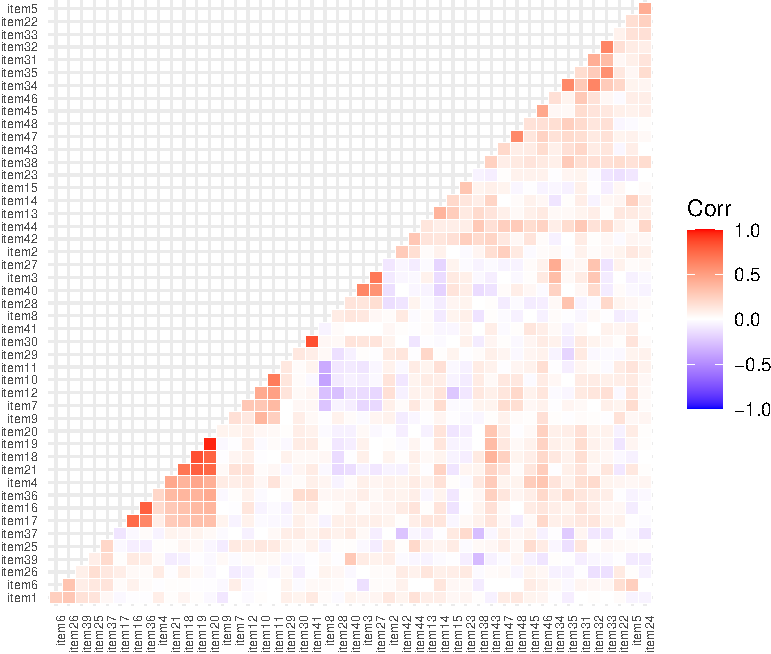
\includegraphics[width=1\linewidth]{manuscript_files/figure-latex/figCorAppB-1} 

}

\caption{Correlation plot of the items}(\#fig:figCorAppB)
\end{figure}

\begin{figure}

{\centering 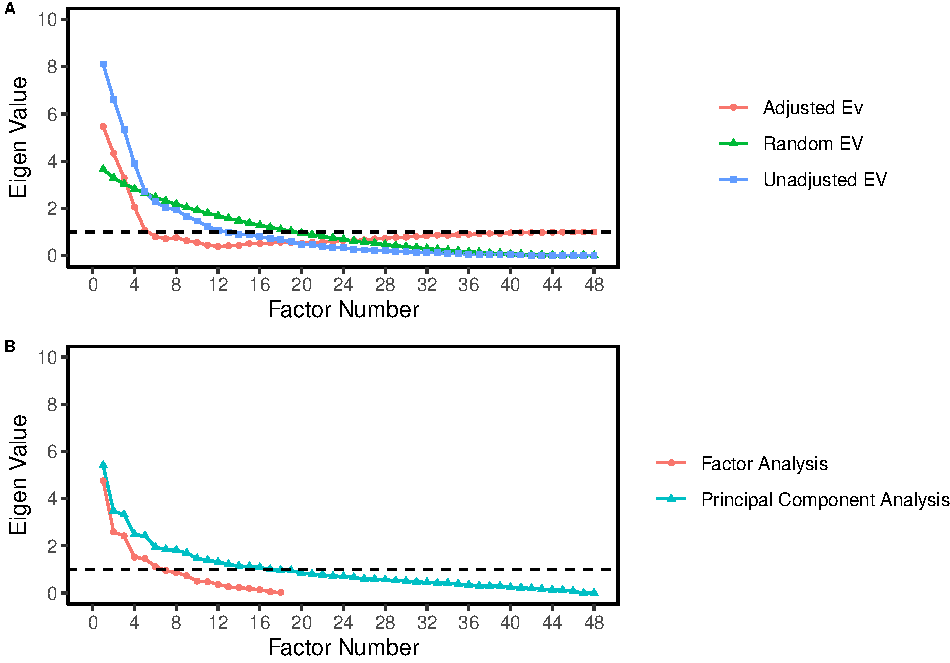
\includegraphics[width=1\linewidth,height=1\textheight]{manuscript_files/figure-latex/facIdFigAppB-1} 

}

\caption{Factor Identification (A) Parallel analysis (B) Scree Plot}(\#fig:facIdFigAppB)
\end{figure}

Horn's parallel analysis with 500 iterations indicated a five-factor
solution. However, Scree plot and the MAP method suggested 6-factor
solution. five-factor solution . As a result, we tested both five-factor
and six-factor solutions.

\begin{table}[h]

\begin{center}
\begin{threeparttable}

\caption{\label{tab:EFATableAppB}Factor loadings and communality of the retained items [Unmerged Responses]}

\small{

\begin{tabular}{ccccccccc}
\toprule
item & \multicolumn{1}{c}{PA1} & \multicolumn{1}{c}{PA2} & \multicolumn{1}{c}{PA5} & \multicolumn{1}{c}{PA3} & \multicolumn{1}{c}{PA4} & \multicolumn{1}{c}{Communality} & \multicolumn{1}{c}{Uniqueness} & \multicolumn{1}{c}{Complexity}\\
\midrule
item19 & 0.99 &  &  &  &  & 1.01 & -0.01 & 1.06\\
item20 & 0.91 &  &  &  &  & 0.87 & 0.13 & 1.11\\
item18 & 0.82 &  &  &  &  & 0.71 & 0.29 & 1.12\\
item21 & 0.8 &  &  &  &  & 0.68 & 0.32 & 1.16\\
item4 & 0.47 &  &  &  &  & 0.25 & 0.75 & 1.30\\
item11 &  & 0.83 &  &  &  & 0.69 & 0.31 & 1.01\\
item10 &  & 0.81 &  &  &  & 0.67 & 0.33 & 1.03\\
item12 &  & 0.56 &  &  &  & 0.37 & 0.63 & 1.37\\
item8 &  & -0.44 &  &  &  & 0.21 & 0.79 & 1.11\\
item7 &  & 0.42 &  &  &  & 0.23 & 0.77 & 1.61\\
item9 &  & 0.33 &  &  &  & 0.12 & 0.88 & 1.10\\
item16 &  &  & 0.95 &  &  & 0.95 & 0.05 & 1.10\\
item17 &  &  & 0.74 &  &  & 0.60 & 0.41 & 1.17\\
item36 & 0.3 &  & 0.73 &  &  & 0.65 & 0.35 & 1.43\\
item3 &  &  &  & 0.85 &  & 0.75 & 0.25 & 1.05\\
item27 &  &  &  & 0.78 &  & 0.62 & 0.38 & 1.03\\
item40 &  &  &  & 0.71 &  & 0.51 & 0.49 & 1.05\\
item35 &  &  &  &  & 0.58 & 0.35 & 0.65 & 1.09\\
item48 &  &  &  &  & 0.57 & 0.35 & 0.65 & 1.14\\
item33 &  &  &  &  & 0.55 & 0.32 & 0.68 & 1.08\\
item47 &  &  &  &  & 0.52 & 0.29 & 0.71 & 1.19\\
item44 &  &  &  &  & 0.45 & 0.22 & 0.78 & 1.15\\
item31 &  &  &  &  & 0.41 & 0.21 & 0.79 & 1.48\\
item38 &  &  &  &  & 0.33 & 0.13 & 0.87 & 1.32\\
\% of Variance & 0.15 & 0.09 & 0.09 & 0.08 & 0.08 & NA & NA & NA\\
\bottomrule
\addlinespace
\end{tabular}

}

\begin{tablenotes}[para]
\normalsize{\textit{Note.} Only loading higher than .30 is reported}
\end{tablenotes}

\end{threeparttable}
\end{center}

\end{table}

\begin{longtable}[]{@{}
  >{\raggedright\arraybackslash}p{(\columnwidth - 0\tabcolsep) * \real{1.00}}@{}}
\toprule
\begin{minipage}[b]{\linewidth}\raggedright
\textbf{Five Factor Solution{[}Unmerged Responses{]} (24 Items)}
\end{minipage} \\
\midrule
\endhead
\textbf{F1} \\
I use light therapy applying a blue light box. \\
I use light therapy applying a light visor. \\
I use light therapy applying a white light box. \\
I use light therapy applying another form of light device. \\
I use an alarm with a dawn simulation light. \\
\textbf{F2} \\
I spend more than 3 hours per day (in total) outside. \\
I spend between 1 and 3 hours per day (in total) outside. \\
I spend as much time outside as possible. \\
I spend 30 minutes or less per day (in total) outside. \\
I go for a walk or exercise outside within 2 hours after waking up. \\
I spend between 30 minutes and 1 hour per day (in total) outside. \\
\textbf{F3} \\
I look at my mobile phone screen immediately after waking up. \\
I use my mobile phone within 1 hour before attempting to fall asleep. \\
I check my phone when I wake up at night. \\
\textbf{F4} \\
I use a blue-filter app on my computer screen within 1 hour before
attempting to fall asleep. \\
I seek out knowledge on how to improve my light exposure. \\
I dim my computer screen within 1 hour before attempting to fall
asleep. \\
I discuss the effects of light on my body with other people. \\
I modify my light environment to match my current needs. \\
I dim my room light within 1 hour before attempting to fall asleep. \\
I use as little light as possible when I get up during the night. \\
\textbf{F5} \\
I wear blue-filtering, orange-tinted, and/or red-tinted glasses indoors
during the day. \\
I wear blue-filtering, orange-tinted, and/or red-tinted glasses outdoors
during the day. \\
I wear blue-filtering, orange-tinted, and/or red-tinted glasses within 1
hour before attempting to fall asleep. \\
\bottomrule
\end{longtable}
\end{appendix}
